% Introduction to Hessians and Quadratic Approximations
% Fall 2021

\qns{Quadratic Approximation Introduction}

\meta{In this problem, we will review the method of second-order approximation, which was introduced in lecture.}

Recall that when dealing with a nonlinear function, we often use local quadratic approximations in order to model the function within a certain neighborhood.

Remember from Taylor approximations that $f(x)\approx f(x_0) + \dfrac{f'(x_0)}{1!} (x - x_0) +   \dfrac{f''(x_0)}{2!} (x - x_0) ^ {2} $.

Applying this to the function $f(x) = x^{3}$, centered at $x = 2$, we get that $f(x)\approx 8 + 12(x - 2) + \dfrac{12(x - 2)^{2}}{2!} = 8 + 12(x - 2) + 6(x - 2)^{2}$.

\begin{center}
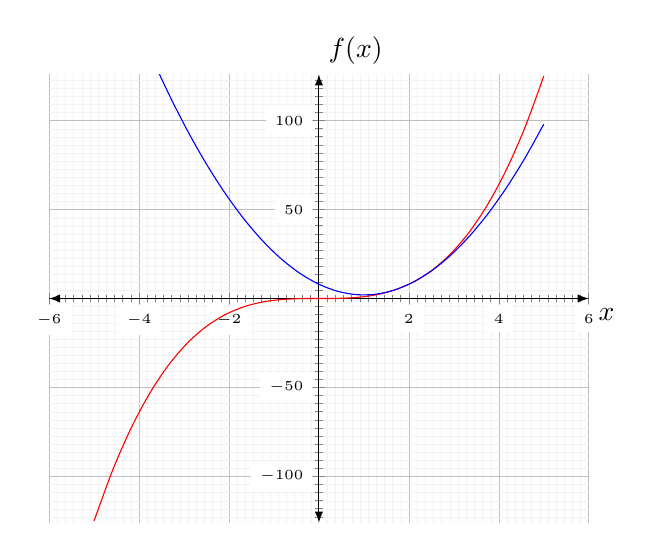
\begin{tikzpicture}
  \begin{axis}[
    xmin=-5,xmax=5,
    ymin=-125,ymax=125,
    grid=both,
    grid style={line width=.1pt, draw=gray!10},
    major grid style={line width=.2pt,draw=gray!50},
    axis lines=middle,
    minor tick num=10,
    enlargelimits={abs=1},
    axis line style={latex-latex},
    ticklabel style={font=\tiny,fill=white},
    xlabel style={at={(ticklabel* cs:1)},anchor=north west},
    ylabel style={at={(ticklabel* cs:1)},anchor=south west},
    xlabel=$x$,
    ylabel=$f(x)$
] 
    \addplot[smooth, red] {x^3}; 
    \addplot[smooth, blue] {8 + 12 * (x - 2) + 6 * (x - 2)^2}; 
  \end{axis}
\end{tikzpicture}
\end{center}


Given this model, we can extend it to multiple dimensions using the concept of the Hessian matrix. Defining the Hessian matrix ${H}$ for a function from 
$\mathbb{R}^{n} \rightarrow \mathbb{R}$ as $f(\vec{x})$, we define the Hessian matrix's entry $H_{ij} = \frac{\partial f}{{\partial x_i}{\partial x_j}}$. Using the same principles for second-order approximation as the single-variable case, we derive that \newline $f(\vec{x})\approx f(\vec{x_0}) + D_x(f) ^ {T} (\vec{x} - \vec{x_0})+ \dfrac{1}{2} (\vec{x} - \vec{x_0})^{T} H_x(f) (\vec{x} - \vec{x_0})$.\newline

\meta{Make sure students understand Clairaut's Theorem.}

Suppose that we examined the function $f(\vec{x}) = \sum_{i=1}^{n} {x_i^{3}} $, where $\vec{x}\in \mathbb{R}^{n}$.  

\begin{enumerate}

\qitem
Compute element $ij$ of the Hessian matrix. What is the Hessian of $f$?

\sol{

  $\frac{\partial f}{\partial x_i} = 3x_i^{2}$

  There are two cases now, $ i = j $ or $ i \neq j $.

  If $ i \neq j $, then $\frac{\partial f}{{\partial x_i}{\partial x_j}} = \frac{\partial}{\partial x_j} (3x_i^{2}) = 0$.

  If $ i = j $, then $\frac{\partial f}{\partial x_i^{2}} = \frac{\partial}{\partial x_i} (3x_i^{2}) = 6x_i$.
  
  Thus, the Hessian is $6x_i$ across the diagonals, $0$ everywhere else.
}

\qitem
Assume n = 3. Compute the second order approximation of $f$ about $\vec{x} = \begin{bmatrix}1 & 1 & 1\end{bmatrix}^{T}$.

\sol{
  Applying the Hessian derived earlier, we get that:
  $H_x(f) = \begin{bmatrix}6 & 0 & 0 \\ 0 & 6 & 0 \\ 0 & 0 & 6 \end{bmatrix} = 6{I}.$\newline

  The gradient is: 

  $\frac{\partial f}{\partial x_i} = 3x_i^{2}$. So, $D_x(f) = \begin{bmatrix} 3 & 3 & 3 \end{bmatrix}^{T}.$\newline

  Finally, $f(\vec{x_0}) = 3(1^{3}) = 3.$\newline  

  Thus, the approximation is: 

  $f(\vec{x})\approx 3 + \begin{bmatrix} 3 & 3 & 3 \end{bmatrix} (\vec{x} - \vec{x_0}) + \frac{1}{2} (\vec{x} - \vec{x_0})^{T} 6{I} (\vec{x} - \vec{x_0})$.\newline 

  This means:
  $f(\vec{x})\approx 3 + \begin{bmatrix} 3 & 3 & 3 \end{bmatrix} (\vec{x} - \vec{x_0}) + 3 (\vec{x} - \vec{x_0})^{T} (\vec{x} - \vec{x_0})$.
}

\qitem

Use your previous approximation to approximate the value of $f$ at $\vec{x} = \begin{bmatrix} 2 & 1 & 2 \end{bmatrix}^{T}$.

\sol {

  Using $f(\vec{x})\approx 3 + \begin{bmatrix} 3 & 3 & 3 \end{bmatrix} (\vec{x} - \vec{x_0}) + 3 (\vec{x} - \vec{x_0})^{T} (\vec{x} - \vec{x_0})$, we get that:\newline

  $(\vec{x} - \vec{x_0}) = \begin{bmatrix} 1 & 0 & 1 \end{bmatrix}^{T}$.

  So, $3 + \begin{bmatrix} 3 & 3 & 3 \end{bmatrix} \begin{bmatrix} 1 \\ 0 \\ 1 \end{bmatrix} + 3 \begin{bmatrix} 1 & 0 & 1 \end{bmatrix} \begin{bmatrix} 1 \\ 0 \\ 1 \end{bmatrix} = 15.$

  so, $f(\vec{x})\approx 15.$
}

\end{enumerate}

